%% For double-blind review submission
%\documentclass[sigplan,review,anonymous]{acmart}
%% For single-blind review submission
%\documentclass[sigplan,review]{acmart}
%% For proofreading
% \documentclass[sigplan,authordraft]{acmart}
%% For final camera-ready submission
\documentclass[sigplan]{acmart}
%% For booklet
% \documentclass[acmsmall]{acmart}

% !TEX root=../main.tex


%% Basics %%%%%%%%%%%%%%%%%%%%%%%%%%%%%%%%%%%%%%%%%%%%%%%%%%%%%%%%%%%%%%%%%%%%%%

%% Fixes %%

\usepackage{underscore}


%% Fonts %%

\usepackage[utf8]{inputenc}
\usepackage[T1]{fontenc}

\usepackage{stmaryrd}

% \usepackage{tgpagella}
% \usepackage{lucidabr}
\usepackage{libertine}
\usepackage[varqu]{zi4}
\usepackage[libertine]{newtxmath}


%% Programming %%

\usepackage{ifthen}


%% Layout %%

% \usepackage[final]{microtype}


%% Additions %%%%%%%%%%%%%%%%%%%%%%%%%%%%%%%%%%%%%%%%%%%%%%%%%%%%%%%%%%%%%%%%%%%

%% Textual %%

\usepackage{paralist}
\usepackage{quoting}


%% Maths %%

\usepackage{amsmath}
\usepackage{mathpartir}


%% Graphics %%

\usepackage{graphicx}
% \usepackage{xcolor}


%% Tabulations %%

\usepackage{booktabs}
\usepackage{array}


%% Listings %%

% \usepackage[final]{listings}


%% References %%

\usepackage{cleveref}

% !TEX root=../main.tex


%% Fixes %%

\frenchspacing

%% NOTE: uses the same lengths as in `tufte-common.def` and `article.cls`...
\setlength{\bigskipamount}   {3.25ex plus .2ex} %% ...before (sub)section
\setlength{\medskipamount}   {2.3ex  plus .2ex} %% ...after section
\setlength{\smallskipamount} {1.5ex  plus .2ex} %% ...after subsection


%% Numbering %%

% \setcounter{secnumdepth}{2}


%% Compact lists %%
%% NOTE: requires `paralist`

\setlength{\pltopsep}{\smallskipamount}
\setlength{\plpartopsep}{\parskip}
\setlength{\plitemsep}{\parskip}
\setlength{\plparsep}{\parskip}

% !TEX root=../main.tex


%% Helpers %%%%%%%%%%%%%%%%%%%%%%%%%%%%%%%%%%%%%%%%%%%%%%%%%%%%%%%%%%%%%%%%%%%%%

\let\newoperator\DeclareMathOperator


%% Text %%%%%%%%%%%%%%%%%%%%%%%%%%%%%%%%%%%%%%%%%%%%%%%%%%%%%%%%%%%%%%%%%%%%%%%%

\newcommand*{\alert}[1]
  {\textbf{#1}}
\newcommand*{\enquote}[1]
  {``#1''}
\newcommand*{\todo}[1]
  {\ensuremath{\star}\marginnote{\ensuremath{\star}#1}}


%% Lists %%
%% NOTE: requires `paralist`

%% Use compact lists by default
\renewenvironment{itemize}
  {\begin{compactitem}}
  {\end{compactitem}}
\renewenvironment{enumerate}
  {\begin{compactenum}}
  {\end{compactenum}}
\renewenvironment{description}
  {\begin{compactdesc}}
  {\end{compactdesc}}
%% Define starred versions as in-paragraph-lists
\newenvironment{itemize*}
  {\begin{inparitem}}
  {\end{inparitem}}
\newenvironment{enumerate*}
  {\begin{inparenum}}
  {\end{inparenum}}
\newenvironment{description*}
  {\begin{inpardesc}}
  {\end{inpardesc}}


%% Blocks %%

\newenvironment{block}
  {\smallskip}
  {\smallskip}


%% Column types %%
%% NOTE: requires `array`

\newcolumntype{L}{>{$}l<{$}}
\newcolumntype{C}{>{$}c<{$}}
\newcolumntype{R}{>{$}r<{$}}
\newcolumntype{T}{>{\ttfamily}l}
\newcolumntype{S}{>{\sffamily}l}


%% References %%
%% NOTE: requires `cleveref`

\let\see\cref
\let\See\Cref
\let\at\cpageref


%% Citations %%
%% NOTE: requires `natbib`

\let\cite\citep
\let\textcite\citet


%% Math %%%%%%%%%%%%%%%%%%%%%%%%%%%%%%%%%%%%%%%%%%%%%%%%%%%%%%%%%%%%%%%%%%%%%%%%

%% NOTE: change this to \emptyset when using a font that includes a nice standard emptyset
\let\nothing\varnothing


%% Braces %%

\let\<\langle
\let\>\rangle

\newcommand*{\llbrace}
  {\{\!|}
\newcommand*{\rrbrace}
  {|\!\}}


%% Operators %%

\let\lt<
\let\gt>
\let\eq\equiv

\newcommand*{\pp}
  {+\!\!+}


%% Shortcuts %%

\newcommand*{\powerset}
  {\mathcal{P}}

\newcommand*{\NN}{\mathbb{N}}
\newcommand*{\ZZ}{\mathbb{Z}}
\newcommand*{\RR}{\mathbb{R}}
\newcommand*{\CC}{\mathbb{C}}

\newcommand*{\LL}{\mathbb{L}}
\newcommand*{\UU}{\mathbb{U}}
\newcommand*{\BB}{\mathbb{B}}
\renewcommand*{\SS}{\mathbb{S}}

\newoperator{\downto}
  {\;\rightarrow\!\shortmid\;}

\let\to\rightarrow
\let\implies\Rightarrow
\let\infers\vdash

% !TEX root=../main.tex


%% Styles %%%%%%%%%%%%%%%%%%%%%%%%%%%%%%%%%%%%%%%%%%%%%%%%%%%%%%%%%%%%%%%%%%%%%%

\lstdefinestyle{natural}
  {columns=fullflexible
  ,gobble=2
  ,breaklines=true
  ,breakatwhitespace=true
  ,literate=
    %{.}{{$\cdot$}}1
    %{.}{{\ }}1
    {<<}{{$\<$}}1
    {>>}{{$\>$}}1
    {->}{{$\to$\ }}2
    % {--}{{--}}1
    %{_}{{\ }}1
    %{\ "}{{\ \textquotedblleft}}2
    %{"\ }{{\textquotedblright\ }}2
  ,basicstyle={\sffamily}
  ,keywordstyle=[1]{\bfseries}
  ,keywordstyle=[2]{\scshape}
  ,keywordstyle=[3]{}
  %,commentstyle={\itshape}
  %,identifierstyle={\itshape}
  ,emphstyle={\itshape}
  %,stringstyle={\rmfamily}
  ,showstringspaces=false
  ,texcl=true
  ,mathescape=true
  %,escapechar=\$
  %,escapeinside={\{\}}
  ,xleftmargin=1\parindent
  }

\lstdefinestyle{flexible}
  {columns=flexible
  ,gobble=2
  ,fontadjust=true
  ,basicstyle={\ttfamily\small}
  ,commentstyle={\itshape}
  ,keywordstyle={\bfseries}
  %,identifierstyle={\itshape}
  %,stringstyle={\ttfamily}
  ,emphstyle={\itshape}
  ,showstringspaces=false
  ,texcl=true
  ,mathescape=true
  %,escapechar=\$
  %,escapeinside={\{\}}
  ,xleftmargin=1\parindent
  }

\lstdefinestyle{literate}
  {literate=
    {\\}{{$\lambda$}}1
    {\\\$}{{\$}}1 %NOTE: otherwise eaten by `\`, NOTE: prevents \$ to be parsed as math escape
    {\\/}{{$\vee$}}1
    {/\\}{{$\wedge$}}1
    {A.}{{$\forall$}}1
    {E.}{{$\exist$}}1
    {->}{{$\rightarrow$ }}1
    {<-}{{$\leftarrow$}}1
    {<=}{{$\leq$}}1
    {>=}{{$\geq$}}1
    {>>=}{{>>=}}3 %NOTE: otherwise eaten by `>=`
    {\{|}{{$\{\!|\!$}}1
    {|\}}{{$\!|\!\}$}}1
    {\{|*|\}}{{$\{\!|\!\!\star\!\!|\!\}$}}3
  }


%% Definitions %%%%%%%%%%%%%%%%%%%%%%%%%%%%%%%%%%%%%%%%%%%%%%%%%%%%%%%%%%%%%%%%%

%% Tasks %%

\lstdefinelanguage{tasks}
  {sensitive=true
  ,morekeywords=[1]{if,then,else,case,of}
  ,morekeywords=[2]{Bool,Int,String,Store,List}
  ,morestring=[b]"
  ,morecomment=[l]--
  ,morecomment=[n]{\{-}{-\}}
  }[keywords,strings,comments]
\lstdefinestyle{tasks}
  {style=natural
  ,literate=
    {\\}{{$\lambda$}}1
    {>>=}{{$\Then$\ }}1
    {>>?}{{$\Next$\ }}1
    {<&>}{{$\And$\ }}1
    {<|>}{{$\Or$\ }}1
    {<?>}{{$\Xor$\ }}1
    {edit}{{$\Edit$}}1
    {enter}{{$\Enter$}}1
    {store}{{$\Change$}}1
    {fail}{{$\Fail$}}1
    {==}{{$\equiv$\ }}1
    {/=}{{$\nequiv$\ }}1
  }

\lstnewenvironment{TASK}[1][]
  {\lstset{language=tasks,style=tasks,#1}}
  {}
\newmacro{TS}[1][1]
  {\lstinline[language=tasks,style=tasks,#1]}
\newmacro{includeTASK}[2][]
  {\lstinputlisting[language=tasks,style=tasks,#1]{#2}}


%% Flows %%

\lstdefinelanguage{flows}
  {sensitive=true
  ,morekeywords=[1]{module,where,define,using,as,yielding,share,holding,with,do,for,fork,then,when,next,done,on,and,or,not,readonly,writeonly,readwrite}
  ,morekeywords=[2]{Bool,Int,String,Shared,List, Date,Document,Photo, Citizen,Company,Declaration}
  ,morekeywords=[3]{True,False,Just,Nothing,List}
  ,morestring=[b]"
  ,morecomment=[l]--
  ,morecomment=[n]{\{-}{-\}}
  }[keywords,strings,comments]

% \lstMakeShortInline[language=flows,style=natural] | % |
\lstnewenvironment{FLOW}[1][]
  {\lstset{language=flows,style=natural,#1}}
  {}
\newmacro{FL}[1][1]
  {\lstinline[language=flows,style=natural,#1]}
\newmacro{includeFLOW}[2][]
  {\lstinputlisting[language=flows,style=natural,#1]{#2}}


%% Clean %%

\lstdefinelanguage{clean}
  {sensitive=true
  %,alsoletter={ABCDEFGHIJKLMNOPQRSTUVWXYZabcdefghijklmnopqrstuvwxyz_`}
  %,alsoletter={~!@\#$\%^\&*-+=?<>:|\\} %$
  ,morekeywords={from,definition,implementation,import,module,system,code,inline,if,case,of,let,let!,in,where,with,class,instance,generic,derive,dynamic,infix,infixl,infixr}
  ,morestring=[b]"
  ,morestring=[b]'
  ,morecomment=[l]//
  ,morecomment=[n]{/*}{*/}
  }[keywords,strings,comments]

\lstnewenvironment{CLEAN}[1][]
  {\lstset{language=clean,style=flexible,#1}}
  {}
\newmacro{CL}[1][1]
  {\lstinline[language=clean,style=flexible,#1]}
\newmacro{includeCLEAN}[2][1]
  {\lstinputlisting[language=clean,style=flexible,#1]{#2}}


\newlogo[ITASKS]{iTasks}
\newlogo{BPMN}
\newlogo{BPEL}
\newlogo{UML}
\newlogo{WFN}

\newlogo{EDSL}
\newlogo{GUI}

\newlogo{STW}
\newlogo{NWO}

% !TEX root=../main.tex



%% Host language %%%%%%%%%%%%%%%%%%%%%%%%%%%%%%%%%%%%%%%%%%%%%%%%%%%%%%%%%%%%%%%


\newkeyword[IF]  {if}
\newkeyword[THEN]{then}
\newkeyword[ELSE]{else}

\newkeyword[Let]{let}
\newkeyword[In]{in}

\newkeyword[Ref] {ref}


\newmacro{If}[3]
  {\IF #1 \THEN #2 \ELSE #3}



%% Values %%


\newmathcommand{unit}{\<\>}


\newvalue{True}
\newvalue{False}
\newvalue[Not]{not}


\newmacro{str}[1]
  {\text{``#1''}}

\newoperator{Length}{\mathrm{length}}


\newvalue[Map]{map}
\newvalue[Fst]{fst}
\newvalue[Snd]{snd}
\newvalue[Assoc]{assoc}



%% Types %%


\newtype{Unit}
\newtype{Bool}
\newtype{Nat}
\newtype{Int}
\newtype{String}
\newtype[Reference]{Ref}
\newtype{Task}
\newtype{Maybe}

\newtype{Euro}



%% Object language %%%%%%%%%%%%%%%%%%%%%%%%%%%%%%%%%%%%%%%%%%%%%%%%%%%%%%%%%%%%%


\let\And\relax
\newoperator{Then}  {\blacktriangleright}
\newoperator{Next}  {\vartriangleright}
\newoperator{And}   {\Join}
\newoperator{Or}    {\blacklozenge}
\newoperator{Xor}   {\lozenge}
\newoperator{Edit}  {\square}
\newoperator{View}  {\overline{\square}}
\newoperator{Enter} {\boxtimes}
\newoperator{Update}{\blacksquare}
\newoperator{Watch} {\overline{\blacksquare}}
\newoperator{Fail}  {\lightning}

\newoperator{AndOr} {\DEPRECATED}



%% Events %%


\newvalue[Left]   {L}
\newvalue[Right]  {R}


\newvalue[Clear]   {C}
\newvalue[Continue]{N}
\newvalue[Pick]    {P}


\newvalue[First]  {F}
\newvalue[Second] {S}
\newvalue[Here]   {H}



%% Semantic functions %%%%%%%%%%%%%%%%%%%%%%%%%%%%%%%%%%%%%%%%%%%%%%%%%%%%%%%%%%


\newmathcommand{evaluate}[rel]
  {\;\downarrow\;}
\newmathcommand{normalise}[rel]
  % {\;\rightarrow\!\shortmid\;}
  {\;\Downarrow\;}
\newmacro{handle}[1]
  {\mathrel{\;\xrightarrow{\;#1\;}\;}}
\newmacro{drive}[1]
  {\mathrel{\;\xRightarrow{\;#1\;}\;}}


\newmathcommand{Value}[cal]
  {V}
\newmathcommand{Firsts}[cal]
  {F}
\newmathcommand{Interface}[cal]
  {U}
\newmathcommand{Succeeding}[cal]
  {S}



%% Depricated %%%%%%%%%%%%%%%%%%%%%%%%%%%%%%%%%%%%%%%%%%%%%%%%%%%%%%%%%%%%%%%%%%

\newvalue[Execute] {<depricated>}

% !TEX root=pldi2019.tex


%% Helpers %%%%%%%%%%%%%%%%%%%%%%%%%%%%%%%%%%%%%%%%%%%%%%%%%%%%%%%%%%%%%%%%%%%%%

\newmacro{newrule}[4][2]
  {\newmacro{#1}{\inferrule*[lab={#1},right={$#2$}]
    {#3}
    {#4}}}
\newmacro{userule}
  {\usemacro}
\newmacro{refrule}[1]
  {\ifthenelse{\isundefined{#1}}
    {\GenericError{}{Rule `#1` is not defined}{}{}}
    {\textsc{#1}}}


\newif\ifstateful
\statefulfalse
\newmacro{st}[2][1]
  {\ifthenelse{\isempty{#1}}
    {\ifstateful{,\:s#2}\else{}\fi}
    {\ifstateful{,\:[#1]s#2}\else{}\fi}}
\newmacro{St}[1]
  {\ifstateful{,\:\Sigma#1}\else{}\fi}



%% Typing %%%%%%%%%%%%%%%%%%%%%%%%%%%%%%%%%%%%%%%%%%%%%%%%%%%%%%%%%%%%%%%%%%%%%%


\newmacro{RelationT}
  {\Gamma,\Sigma \infers e : \tau}


\newrule{T-Var}
  {x:\tau\in\Gamma}
  {\Gamma,\Sigma\infers x:\tau}


\newrule{T-Abs}
  {\Gamma[x:\tau_1] ,\Sigma \infers e:\tau_2}
  {\Gamma,\Sigma \infers \lambda x : \tau_1 . e :\tau_1 \to \tau_2}

\newrule{T-App}
  {\Gamma,\Sigma \infers e_1:\tau_1\to\tau_2\\
   \Gamma,\Sigma \infers e_2:\tau_1}
  {\Gamma,\Sigma \infers e_1 e_2 :\tau_2}


\newrule{T-If}
  {\Gamma,\Sigma \infers e_1:\Bool\\
   \Gamma,\Sigma \infers e_2:\tau\\
   \Gamma,\Sigma \infers e_3:\tau}
  {\Gamma,\Sigma \infers \If{e_1}{e_2}{e_3}:\tau}


\newrule{T-Pair}
    {\Gamma,\Sigma \infers e_1 : \tau_1 \\
     \Gamma,\Sigma \infers e_2 : \tau_2}
    {\Gamma,\Sigma \infers \tuple{e_1, e_2} :\tau_1 \times \tau_2}


\newrule{T-Ref}
  {\Gamma,\Sigma \infers e:\tau}
  {\Gamma,\Sigma \infers \Ref e :\Reference \tau}

\newrule{T-Deref}
  {\Gamma,\Sigma \infers e:\Reference \tau}
  {\Gamma,\Sigma\infers\ !e:\tau}

\newrule{T-Assign}
  {\Gamma,\Sigma\infers e_1:\Reference \tau\\
   \Gamma,\Sigma\infers e_2:\tau}
  {\Gamma,\Sigma\infers e_1 := e_2:\Unit}

\newrule{T-Loc}
  {\Sigma(l) = \tau}
  {\Gamma,\Sigma\infers l:\Reference \tau}


\newrule{T-Edit}
  {\Gamma,\Sigma \infers e : \tau}
  {\Gamma,\Sigma \infers \Edit e : \Task \tau}

\newrule{T-Fill}
  {\ }
  {\Gamma,\Sigma \infers \Enter \tau : \Task \tau}

\newrule{T-Update}
  {\Gamma,\Sigma \infers e : \Reference \tau}
  {\Gamma,\Sigma \infers \Update e : \Task \tau}


\newrule{T-Fail}
  {\ }
  {\Gamma,\Sigma \infers \Fail : \Task \tau}


\newrule{T-Then}
  {\Gamma,\Sigma \infers e_1 : \Task \tau_1 \\
   \Gamma,\Sigma \infers e_2 : \tau_1 \to \Task \tau_2}
  {\Gamma,\Sigma \infers e_1 \Then e_2 : \Task \tau_2}


\newrule{T-Next}
  {\Gamma,\Sigma \infers e_1 : \Task \tau_1 \\
   \Gamma,\Sigma \infers e_2 : \tau_1 \to \Task \tau_2}
  {\Gamma,\Sigma \infers e_1 \Next e_2 : \Task \tau_2}


\newrule{T-And}
  {\Gamma,\Sigma \infers e_1 : \Task \tau_1 \\
   \Gamma,\Sigma \infers e_2 : \Task \tau_2}
  {\Gamma,\Sigma \infers e_1 \And e_2 : \Task\,(\tau_1 \times \tau_2)}


\newrule{T-Or}
  {\Gamma,\Sigma \infers e_1 : \Task \tau \\
   \Gamma,\Sigma \infers e_2 : \Task \tau }
  {\Gamma,\Sigma \infers e_1 \Or e_2 : \Task \tau}


\newrule{T-Xor}
  {\Gamma,\Sigma \infers e_1 : \Task \tau \\
   \Gamma,\Sigma \infers e_2 : \Task \tau }
  {\Gamma,\Sigma \infers e_1 \Xor e_2 : \Task \tau}


\newrule{T-Appoint}
  {\Gamma,\Sigma\infers e:\Task\tau}
  {\Gamma,\Sigma\infers u \At e:\Task\tau}



%% Evaluation %%%%%%%%%%%%%%%%%%%%%%%%%%%%%%%%%%%%%%%%%%%%%%%%%%%%%%%%%%%%%%%%%%


\newmacro{RelationE}
  {e,s \evaluate v,s'}


\newrule{E-Value}[v\in\set{\lambda x:\tau.e, \unit, l, B, I, S}]
  {\ }
  {v,s\evaluate v,s}

\newrule{E-App}
  {e_1,s\evaluate \lambda x:\tau.e_1',s'\\
   e_2,s'\evaluate v_2,s''\\
   e_1'[x\mapsto v_2],s''\evaluate v_1,s'''}
  {e_1 e_2,s \evaluate v_1,s'''}


\newrule{E-IfTrue}
    {e_1,s\evaluate \True,s'\\
     e_2,s'\evaluate v,s''}
    {\If{e_1}{e_2}{e_3},s\evaluate v,s''}

\newrule{E-IfFalse}
  {e_1,s\evaluate \False,s'\\
   e_3,s'\evaluate v,s''}
  {\If{e_1}{e_2}{e_3},s\evaluate v,s''}


\newrule{E-Pair}
  {e_1,s\evaluate v_1,s'\\
   e_2,s'\evaluate v_2,s''}
  {\tuple{e_1,e_2},s\evaluate\tuple{v_1,v_2},s''}


\newrule{E-Ref}
  {e,s\evaluate v,s'\\
   l\not\in Dom(s)}
  {\Ref e,s\evaluate l,s'[l\mapsto v]}

\newrule{E-Deref}
  {e,s\evaluate l,s'}
  {!e,s\evaluate s'(l),s'}

\newrule{E-Assign}
  {e_1,s\evaluate l,s'\\
   e_2,s'\evaluate v_2,s''}
  {e_1:=e_2,s\evaluate \unit,s''[l\mapsto v_2]}


\newrule{E-Sequence}
  {?}
  {e_1;e_2 \evaluate ?}

\newrule{E-Edit}
  {e,s \evaluate v,s'}
  {\Edit e , s\evaluate \Edit v,s'}

\newrule{E-Fill}
  {\ }
  {\Enter \tau,s \evaluate \Enter \tau,s}

\newrule{E-Update}
  {e,s\evaluate l,s'}
  {\Update e ,s\evaluate \Update l,s'}


\newrule{E-Fail}
  {\ }
  {\Fail,s \evaluate \Fail,s}


\newrule{E-Then}
  {e_1 ,s\evaluate t_1,s'}
  {e_1 \Then e_2,s \evaluate t_1 \Then e_2,s'}

\newrule{E-Next}
  {e_1 ,s\evaluate t_1,s'}
  {e_1 \Next e_2 ,s\evaluate t_1 \Next e_2,s'}


\newrule{E-And}
  {e_1 ,s\evaluate t_1 ,s'\\
   e_2 ,s'\evaluate t_2,s''}
  {e_1 \And e_2 ,s\evaluate t_1 \And t_2,s''}


\newrule{E-Or}
  {e_1 ,s\evaluate t_1 ,s'\\
   e_2 ,s'\evaluate t_2,s''}
  {e_1 \Or e_2 ,s\evaluate t_1 \Or t_2,s''}

\newrule{E-Xor}
  {\ }
  {e_1 \Xor e_2 ,s\evaluate e_1 \Xor e_2,s}


\newrule{E-Appoint}
    {e,s\evaluate t,s'}
    {u \At e,s\evaluate u \At t,s'}



%% Normalisation %%%%%%%%%%%%%%%%%%%%%%%%%%%%%%%%%%%%%%%%%%%%%%%%%%%%%%%%%%%%%%%


\newmacro{RelationS}
  {t,s \stride t',s'}


\newrule{S-Edit}
  { }
  {\Edit v,s \stride \Edit v,s}

\newrule{S-Fill}
  { }
  {\Enter \tau,s \stride \Enter \tau,s}

\newrule{S-Update}
  { }
  {\Update l,s \stride \Update l,s}


\newrule{S-Fail}
  { }
  {\Fail,s \stride \Fail,s}


\newrule{S-ThenStay}[\Value(t_1',s') = \bot]
  {t_1,s \stride t_1',s'}
  {t_1 \Then e_2,s \stride t_1' \Then e_2,s'}

\newrule{S-ThenFail}[\Value(t_1',s') = v_1 \land \Failing(t_2,s'')]
  {t_1,s \stride t_1',s' \\
   e_2\ v_1,s' \evaluate t_2,s''}
  {t_1 \Then e_2,s \stride t_1' \Then e_2,s'}

\newrule{S-ThenCont}[\Value(t_1',s') = v_1 \land \lnot\Failing(t_2,s'')]
  {t_1,s \stride t_1',s' \\
   e_2\ v_1,s' \evaluate t_2 ,s'' \\
   t_2,s'' \stride t_2',s'''}
  {t_1 \Then e_2,s \stride t_2',s'''}

\newrule{S-Next}
  {t_1,s \stride t_1',s'}
  {t_1 \Next e_2,s \stride t_1' \Next e_2,s'}


\newrule{S-And}
  {t_1,s  \stride t_1',s' \\
   t_2,s' \stride t_2',s''}
  {t_1 \And t_2,s \stride t_1' \And t_2',s''}


\newrule{S-OrLeft}[\Value(t_1',s') = v_1]
  {t_1,s  \stride t_1',s'}
  {t_1 \Or t_2,s \stride t_1',s'}

\newrule{S-OrRight}[\Value(t_1',s') = \bot \land \Value(t_2',s'') = v_2]
  {t_1,s  \stride t_1',s' \\
   t_2,s' \stride t_2',s''}
  {t_1 \Or t_2,s \stride t_2',s''}

\newrule{S-OrNone}[\Value(t_1',s') = \bot \land \Value(t_2',s'') = \bot]
  {t_1,s  \stride t_1',s' \\
   t_2,s' \stride t_2',s''}
  {t_1 \Or t_2,s \stride t_1' \Or t_2',s''}


\newrule{S-Xor}
  { }
  {e_1 \Xor e_2,s \stride e_1 \Xor e_2,s}

\newrule{S-Eval}[e \neq e']
    {e,s \evaluate e',s' \\
     e',s' \stride e'',s''}
    {e,s \stride e'',s''}


\newrule{S-Appoint}
  {t,s\stride t',s'}
  {u \At t,s\stride u \At t',s'}


% \newrule{S-Next}[t_1' = \Edit v]
%   {t_1,\Sigma \stride t_1'\st{'}   \\
%    e\ v \evaluate t_2       \\
%    t_2\st{'} \stride t_2'\st{''} }
%   {t_1 \Next e,\Sigma \stride t_2'\st{''}}

% \newrule{S-NextEval}
%   {e_1,\Sigma \stride u_1\st{'}}
%   {e_1 \Next e_2,\Sigma \stride u_1 \Next e_2\st{'}}




%% Normalisation %%


\newmacro{RelationN}
  {e,s \normalise t,s'}


\newrule{N-Done}[\Dirty(s,s'') \cap \Watching(t') = \nothing]
    {e,s \evaluate t,s' \\
     t,s' \stride t',s''}
    {t,s \normalise t',s''}


\newrule{N-Stride}[\Dirty(s,s'') \cap \Watching(t') \neq \nothing]
    {e,s \evaluate t,s' \\
     t,s' \stride t',s'' \\
     t',s'' \normalise t'',s'''}
    {e,s \normalise t'',s''}



%% Handling %%


\newmacro{RelationH}
  {t,s \handle{i} t',s'}

\newrule{H-Change}[v, v' : \tau]
  { }
  {\Edit v,s \handle{v'} \Edit v',s}

\newrule{H-Empty}[v : \tau]
  { }
  {\Edit v,s \handle{\Empty} \Enter \tau,s}

\newrule{H-Fill}[v' : \tau]
  { }
  {\Enter \tau,s \handle{v'} \Edit v',s}

\newrule{H-Update}[s(l), v' : \tau]
  { }
  {\Update l,s \handle{v'} \Update l,s[l \mapsto v']{}}


\newrule{H-PassThen}
  {t_1,s \handle{i} t_1',s'}
  {t_1 \Then e_2,s \handle{i} t_1' \Then e_2,s'}

\newrule{H-PassNext}
  {t_1,s \handle{i} t_1',s'}
  {t_1 \Next e_2,s \handle{i \neq \Continue} t_1' \Next e_2,s'}

\newrule{H-Next}[\Value{(t_1,s)}\equiv v_1 \wedge \neg\Failing{(t_2,s')}]
  {e_2 v_1,s\stride t_2,s'}
  {t_1 \Next e_2,s \handle{\Continue} t_2,s'}


\newrule{H-FirstAnd}
  {t_1,s \handle{i} t_1',s' }
  {t_1 \And t_2,s \handle{\First i} t_1' \And t_2,s'}

\newrule{H-SecondAnd}
  {t_2,s \handle{i} t_2',s'}
  {t_1,s \And t_2 \handle{\Second i} t_1 \And t_2',s'}


\newrule{H-FirstOr}
  {t_1,s \handle{i} t_1',s'}
  {t_1 \Or t_2,s \handle{\First i} t_1' \Or t_2,s'}

\newrule{H-SecondOr}
  {t_2,s \handle{i} t_2',s' }
  {t_1 \Or t_2,s \handle{\Second i} t_1 \Or t_2',s'}


\newrule{H-PickLeft}[e_1,s\evaluate t_1,s'\wedge \neg\Failing(t_1,s')]
  { }
  {e_1 \Xor e_2,s \handle{\Left} e_1,s}

\newrule{H-PickRight}[e_2,s\evaluate t_2,s'\wedge \neg\Failing(t_2,s')]
  { }
  {e_1 \Xor e_2,s \handle{\Right} e_2,s}


\newrule{H-Appoint}
  {t,s \handle{i} t',s'}
  {u \At t,s\handle{i} u \At t',s'}



%%%%


% \newrule{H-Stay'}[\Value(t_1) = \bot]
%   {\ }
%   {t_1 \Next e,\Sigma \handle{\Next} t_1 \Next e,\Sigma}

% \newrule{H-Next'}[\Value(t_1) = v]
%   {e\ v \evaluate t_2    \\
%    t_2,\Sigma \stride t_2'\st{'} }
%   {t_1 \Next e,\Sigma \handle{\Next} t_2'\st{'}}

% \newrule{H-Stay}[\Value(t_1) = \bot]
%   {\ }
%   {t_1 \Then e,\Sigma \handle{\Execute \pi} t_1 \Then e,\Sigma}

% \newrule{H-Fail'}[\Value(t_1) = v \land t_2 = \Fail]
%   {e\ v \evaluate t_2    \\
%    t_2,\Sigma \handle{\Pick \pi} t_2'\st{'} }
%   {t_1 \Then e,\Sigma \handle{\Execute \pi} t_1 \Then e,\Sigma}

% \newrule{H-Next}[\Value(t_1) = v \land t_2 \neq \Fail]
%   {e\ v \evaluate t_2    \\
%    t_2,\Sigma \handle{\Pick \pi} t_2'\st{'} }
%   {t_1 \Then e,\Sigma \handle{\Execute \pi} t_2'\st{'}}

% \newrule{H-PassS}
%   {t_1,\Sigma \handle{i} t_1'\st{'}}
%   {t_1 \Next e,\Sigma \handle{i} t_1' \Next e\st{'}}

% \newrule{H-Pass}[i \neq \Execute \pi]
%   {t_1,\Sigma \handle{i} t_1'\st{'}       \\
%    t_1' \Then e\st{'} \stride t_2\st{''} }
%   {t_1 \Then e,\Sigma \handle{i} t_2\st{''}}

% \newrule{H-Fallback}
%   { }
%   {t,\Sigma \handle{i} t,\Sigma}



%% Driving %%


\newmacro{RelationD}
  {t,s \drive{i} t',s'}


\newrule{D-Handle}
  {t,s \handle{i} t',s' \\
   t',s' \normalise t'',s''}
  {t,s \drive{i} t'',s''}


\acmConference[PLDI'19]
  {International Conference on Programming Language Design and Implementation}
  {June 2019}
  {Phoenix, Arizona, United States}
\acmYear{2019}

%\acmISBN{978-x-xxxx-xxxx-x/YY/MM}
%\acmDOI{10.1145/nnnnnnn.nnnnnnn}

%\startPage{1}

\settopmatter{printfolios=true,printccs=false,printacmref=false}
\setcopyright{none}             %% For review submission
%\setcopyright{acmcopyright}
%\setcopyright{acmlicensed}
%\setcopyright{rightsretained}
%\copyrightyear{2017}           %% If different from \acmYear


%% Bibliography style
\bibliographystyle{ACM-Reference-Format}
%% Citation style
%\citestyle{acmauthoryear}  %% For author/year citations
\citestyle{acmnumeric}      %% For numeric citations
%\setcitestyle{nosort}      %% With 'acmnumeric', to disable automatic
                            %% sorting of references within a single citation;
                            %% e.g., \cite{Smith99,Carpenter05,Baker12}
                            %% rendered as [14,5,2] rather than [2,5,14].
%\setcitesyle{nocompress}   %% With 'acmnumeric', to disable automatic
                            %% compression of sequential references within a
                            %% single citation;
                            %% e.g., \cite{Baker12,Baker14,Baker16}
                            %% rendered as [2,3,4] rather than [2-4].



\begin{document}

%% Title information
\title{Interactive Processes: A Formal Foundation for Task-Oriented Programming}
                                        %% [Short Title] is optional;
                                        %% when present, will be used in
                                        %% header instead of Full Title.
%\titlenote{with title note}             %% \titlenote is optional;
                                        %% can be repeated if necessary;
                                        %% contents suppressed with 'anonymous'
%\subtitle{Revisited edition}            %% \subtitle is optional
%\subtitlenote{with subtitle note}       %% \subtitlenote is optional;
                                        %% can be repeated if necessary;
                                        %% contents suppressed with 'anonymous'


%% Author information
%% Contents and number of authors suppressed with 'anonymous'.
%% Each author should be introduced by \author, followed by
%% \authornote (optional), \orcid (optional), \affiliation, and
%% \email.
%% An author may have multiple affiliations and/or emails; repeat the
%% appropriate command.
%% Many elements are not rendered, but should be provided for metadata
%% extraction tools.

\author{Markus Klinik}
%\authornote{with author1 note}          %% \authornote is optional; can be repeated if necessary
%\orcid{nnnn-nnnn-nnnn-nnnn}             %% \orcid is optional
\affiliation{
  %\position{PhD}
  \department{Department of Software Science}
  %\department{Institute for Computing and Information Sciences}
                                        %% \department is recommended
  \institution{Radboud University}
                                        %% \institution is required
  \streetaddress{Toernooiveld 212}
  \postcode{6525 EC}
  \city{Nijmegen}
  %\state{State1}
  \country{The Netherlands}
}
\email{m.klinik@cs.ru.nl}               %% \email is recommended

\author{Nico Naus}
%\authornote{with author1 note}          %% \authornote is optional; can be repeated if necessary
%\orcid{nnnn-nnnn-nnnn-nnnn}             %% \orcid is optional
\affiliation{
  %\position{PhD}
  \department{Department of Information and Computing Sciences}
                                        %% \department is recommended
  \institution{Utrecht University}      %% \institution is required
  \streetaddress{Princetonplein 5}
  \postcode{3584 CC}
  \city{Utrecht}
  %\state{State1}
  \country{The Netherlands}
}
\email{n.naus@uu.nl}                    %% \email is recommended

\author{Tim Steenvoorden}
%\authornote{with author1 note}          %% \authornote is optional; can be repeated if necessary
%\orcid{nnnn-nnnn-nnnn-nnnn}             %% \orcid is optional
\affiliation{
  %\position{PhD}
  \department{Department of Software Science}
  %\department{Institute for Computing and Information Sciences}
                                        %% \department is recommended
  \institution{Radboud University}      %% \institution is required
  \streetaddress{Toernooiveld 212}
  \postcode{6525 EC}
  \city{Nijmegen}
  %\state{State1}
  \country{The Netherlands}
}
\email{tim@cs.ru.nl}                     %% \email is recommended

% \author{Rinus Plasmeijer}
% %\authornote{with author2 note}       %% \authornote is optional; can be repeated if necessary
% %\orcid{nnnn-nnnn-nnnn-nnnn}             %% \orcid is optional
% \affiliation{
%   %\position{prof.}
%   % \department{Department of Software Science}
%   \department{Institute for Computing and Information Sciences}
%                                         %% \department is recommended
%   \institution{Radboud University}
%                                         %% \institution is required
%   \streetaddress{Toernooiveld 212}
%   \city{Nijmegen}
%   %\state{State1}
%   \postcode{6525 EC}
%   \country{The Netherlands}
% }
% \email{rinus@cs.ru.nl}                  %% \email is recommended


%% Paper note
%% The \thanks command may be used to create a "paper note" ---
%% similar to a title note or an author note, but not explicitly
%% associated with a particular element.  It will appear immediately
%% above the permission/copyright statement.
%\thanks{with paper note}                %% \thanks is optional
                                        %% can be repeated if necesary
                                        %% contents suppressed with 'anonymous'


%% Abstract
%% Must come before \maketitle command
\begin{abstract}
  % !TEX root=../pldi2019.tex

Task-Oriented Programming (\TOP) is a programming paradigm that focusses on modelling real world collaborations between people.
It prescribes a declarative programming style to specify multi-user workflows.
Workflows can be higher-order.
They communicate through typed values on a local or global level.
Such specifications can be turned into interactive applications for different platforms,
supporting collaboration during execution.

In this paper we decompose the rich features of \TOP into elementary language elements,
which makes them suitable for formal treatment.
We use the simply typed lambda calculus, extended with pairs and references, as a base language.
On top of this language, we develop \TOPHAT (TopHat), a calculus for modular interactive workflows.

We describe \TOPHAT by means of a layered semantics.
These layers consist of multiple big step evaluations on expressions,
and two labelled transition systems, handling user inputs.
We show some interesting properties of this machinery.
This approach allows for comparison with other work in the field.
We place \TOPHAT in perspective with the process calculus \CSP.

\end{abstract}

% \begin{teaserfigure}
%    \includegraphics[width=\textwidth]{figures/declrequest-part.pdf}
%    \caption{This is a teaser}
%    \label{fig:teaser}
% \end{teaserfigure}

%% 2012 ACM Computing Classification System (CSS) concepts
%% Generate at 'http://dl.acm.org/ccs/ccs.cfm'.

%% End of generated code


%% Keywords
%% comma separated list, optional
%\keywords{workflow, dataflow, visual programming, program generation}


%% Note: \maketitle command must come after title commands, author
%% commands, abstract environment, Computing Classification System
%% environment and commands, and keywords command.
\maketitle
\statefultrue

% !TEX root=../main.tex



\section{Introduction}

%XXX: Alejandro:
% The introduction seems to be more about why Task-Oriented Programming is nice and useful.
% Personally, I would like it to tell me another story:
% given that some people find TOP useful (as shown by the many examples),
% why should be care about formalising it and which challenges does it pose?
% I think this is what people from ICFP would care about more.
%NOTE: Ik hoop dat de `Challenges` sectie dit wat opvangt. --TS

Many applications these days are developed to support workflows in institutions and businesses.
Take for example expense declarations, order processing, and emergency management.
Some of these workflows occur on the boundary between organisations and customers,
like flight bookings or tax returns.
What they all have in common is
that they need to interact with different people (end users, tax officers, customers, etc.)
and they use information from multiple sources (input forms, databases, sensors, etc.).

\subsection{Tasks}

We call interactive units of work based on information sources \emph{tasks}.
% Tasks stand for units of work in the real world, assigned to people.
Tasks model real world collaboration between users,
are driven by work users do,
and are assigned to some user.
Users could be people out in the field or sitting behind their desks,
as well as machines doing calculations or fetching data.



\subsection{Task-oriented programming}
\label{sec:top}

%XXX: Alejandro: Not entirely convincing
% Hij heeft het hier volgens mij over de titel van de sectie en het woord aims in de eerste zin. Misschien moeten we een hardere claim doen hier? --NN
% Ik heb `aims` vervangen door `targets`. Doet dat wat? --TS

% Task-Oriented Programming (\TOP) is a programming paradigm aimed at writing interactive multi-user applications in a declarative way \cite{conf/ppdp/PlasmeijerLMAK12}.
Task-oriented programming (\TOP) is a programming paradigm which targets the sweet spot between faithful modelling workflows
and rapid prototyping of multi-user web applications supporting these workflows \cite{conf/ppdp/PlasmeijerLMAK12}.
% Task-oriented programming (\TOP) is a programming paradigm to support these ways of working.
\TOP focusses on modelling collaboration patterns.
This gives rise to a user's need to interact and share information.
Next to that, \TOP automatically provides solutions to common development jobs like designing \GUI{s}, connecting to databases, and communicating between servers and clients.

Therefore,
a language that supports \TOP should choose the right level of abstraction to support two things.
% \TOP has two aspects.
% First, it should allow to specify tasks from real world scenarios.
Firstly, it should provide primitive building blocks that are useful for high-level descriptions of how users collaborate,
with each other and with machines.
These building blocks are: \emph{editors}, \emph{composition}, and \emph{shared data}.
% Second, it should be able to generate multi-user web applications to support these scenarios.
Secondly, it should be able to generate applications, including graphical user interfaces, from workflows modelled with said building blocks.

Users can work together in a number of ways, and this is reflected in \TOP by task compositions.
There is \emph{sequential} composition, \emph{parallel} composition, and \emph{choice}.
Users need to communicate in order to engage in these forms of collaboration.
This is reflected in \TOP by three kinds of communication mechanisms.
There is data flow \emph{alongside} control flow, where the result of a task is passed onto the next.
There is data flow \emph{across} control flow, where information is shared between multiple tasks.
Finally, there is communication with the \emph{outside} world, where information is entered into the system via input events.
The end points where the outside world interacts with \TOP applications are called editors.
In generated applications, editors can take many forms, like input fields, selection boxes, or map widgets.



\subsection{Utilisation}


Currently, we know of two frameworks implementing \TOP: \ITASKS and \MTASKS.

\ITASKS is an implementation of \TOP, in the form of a shallowly embedded domain-specific language in the lazy functional programming language Clean.
It is a library that provides editors, monadic combinators, and shared data sources.
\ITASKS uses the generic programming facilities of Clean to derive rich client and server applications from a single source.
It has been used to model an incident management tool for the Dutch coast guard~\cite{conf/iscram/LijnseJP12}.
Also it has been used numerous times to prototype ideas for Command and Control~\cite{theses/nlda/Kool17, theses/radboud/Stutterheim17}, and in a case study for the Dutch tax authority~\cite{conf/sfp/StutterheimAP17}.

\MTASKS is a subset of \ITASKS,
focussing on \IOT devices and deployment on micro controllers.
It has been used to control home thermostats and other home automation applications \cite{koopman2018task}.
%
Both implementations currently lack formal semantics which are suited to prove properties about tasks.



\subsection{Challenges}

% \ITASKS is the de-facto reference implementation of \TOP.
Both \ITASKS and \MTASKS have been designed for developing real-world applications.
They are constantly being extended and improved with this goal in mind.
The different variations of task combinators and the details that come with real-world requirements,
make it hard to see what the essence of \TOP is.
% One of the defining aspects of both \ITASKS and \MTASKS is their embedding in a functional programming language.
% This creates a synergy where they profit from the expressivity of Clean, while enhancing the language with functionality for user interaction.
Also, the tight integration of both frameworks with Clean, makes it difficult to see where the boundaries are.
This makes formal reasoning about \TOP programs impossible.

In this paper, we want to take a step back and look at the spirit of \TOP.
We do this both formally and informally.
Informally in the sense that we give an intuitive description of the features that define task-oriented programming.
Formally in the sense that we develop a calculus which formalises these features as language constructs,
and we give them a semantics in the style that is common in programming language research.
We separate the task layer and the underlying host language, both syntactically and semantically.
Thus making explicit which properties of \TOP come from the task layer, and which come from functional programming.
Our challenge, therefore, is to model the properties of \TOP into a calculus
and pave the way for formal treatment of \TOP programs.
We give this formal calculus the name \TOPHAT (TopHat).



\subsection{Contributions}

Our contributions to workflow modelling, functional programming language design, and rapid application development are as follows.


\begin{itemize}
  \item
    We describe the essential concepts of task-oriented programming.

  \item
    We present a formal calculus for modelling declarative workflows, embedded in a simply typed lambda-calculus, called \TOPHAT.
    It is based on the aforementioned essential \TOP concepts.

  \item
    We develop a layered operational semantics for \TOPHAT that is driven by user input.
    The semantics of the task language is clearly separated from the semantics of the underlying host language.

  \item
    Along with this semantics, we present the following semantic observations on tasks:
    the current value, whether a term is stuck, the current user interface, and the accepted inputs.

  \item
    We prove progress and type preservation for \TOPHAT.

  \item
    Using both the essential concepts and the formal calculus, we compare \TOP with related work in areas ranging from business process modelling, to process algebras and reactive programming.

  \item
    We implemented the whole semantic system in the dependently typed programming language Idris \cite{journals/jfp/Brady13}.

  \item
    To create executable applications, we implemented the task layer of \TOPHAT in iTasks.
    This also demonstrates that the former is a subset of the latter.


\end{itemize}


\subsection{Structure}

In \cref{sec:example} we demonstrate the functionality of \TOPHAT by means of an example,
\Cref{sec:intuition} gives an overview of the essential concepts of \TOP.
\Cref{sec:language} introduces the \TOPHAT calculus syntax
and \cref{sec:semantics} the semantics.
Then in \cref{sec:properties} we show that certain properties hold for the calculus.
We take a look at related work in \cref{sec:relatedwork}
and conclude in \cref{sec:conclusions}.

% !TEX root=../pldi2019.tex

\section{Example}

\lstset{emph={p, ps, ss}}

In this section we develop a small example program to demonstrate the capabilities of \TOPHAT.
The example is a simple flight booking system.
It demonstrates communication with the environment, communication between parallel tasks, synchronisation, and input validation.

The application works as follows.
\begin{enumerate*}
  \item A user has to input a list of passengers for which to book tickets.
  \item At least one of these passengers has to be an adult.
  \item After a valid list of passengers has been input, the user has to pick seats.
  \item Only free seats may be picked.
  \item Every passenger must have exactly one seat.
  \item Multiple users should be able to book tickets at the same time.
\end{enumerate*}
For this example we assume that the host language has lists and two functions on them: intersect and difference.
For brevity, we omit the type annotations of variable bindings.

We start by defining some type aliases.
A passenger is a pair with name and age.
A seat is a pair with a row number and a seat letter.
A booking contains a list of passengers and a list of seats.
\begin{TASK}
  type Passenger = String * Int
  type Seat = Int * String
\end{TASK}

Choosing seats requires reading and updating shared information.
The list of free seats is stored in a reference called \TS{freeSeats}.
\begin{TASK}
  let freeSeats = ref [<<1,"A">>, <<1,"B">>, <<1,"C">>, ...] in
\end{TASK}

The flight booking task starts with entering a valid list of passengers,
denoted by \TS{enter (List Passenger)}.
A passenger is valid if the name is not empty and the age is at least 0.
A list of passengers is valid if each passenger is valid, and at least one of the passengers is an adult.
When the user has entered a valid list of passengers, the step after \TS{>>?} becomes enabled,
and the user can proceed to picking seats.
\begin{TASK}
  let valid = \p. not (fst p == "") /\ snd p >= 0 in
  let adult = \p. snd p >= 18 in
  let allValid = \ps. all valid ps /\ any adult ps in
  let bookFlight = enter (List Passenger) >>? \ps.
    if allValid ps then chooseSeats ps else fail in
\end{TASK}
A selection of seats is correct if every entered seat is free.
\begin{TASK}
  let correct = \ss. intersect ss !freeSeats == ss in
  let chooseSeats = \ps. enter (List Seat) >>? \ss.
    if correct ss /\ length ps == length ss
      then confirmBooking ps ss else fail in
\end{TASK}
The function \TS{confirmBooking} removes the picked seats from the shared list of free seats,
and displays the end result using the \TS{edit}-construct.
\begin{TASK}
  let confirmBooking = \ps. \ss.
    freeSeats := difference !freeSeats ss; edit <<ps, ss>> in
\end{TASK}
% It uses a function \TS{difference}, which removes all elements from the second list from the first list.

The main task appoints the \TS{bookFlight} task to three different users: \TS{u1}, \TS{u2}, and \TS{u3},
and run these tasks in parallel.
%%NOTE: parentheses make the line to long...
\begin{TASK}
  u1 @ bookFlight <&> u2 @ bookFlight <&> u3 @ bookFlight
\end{TASK}

\begin{figure}[h]
  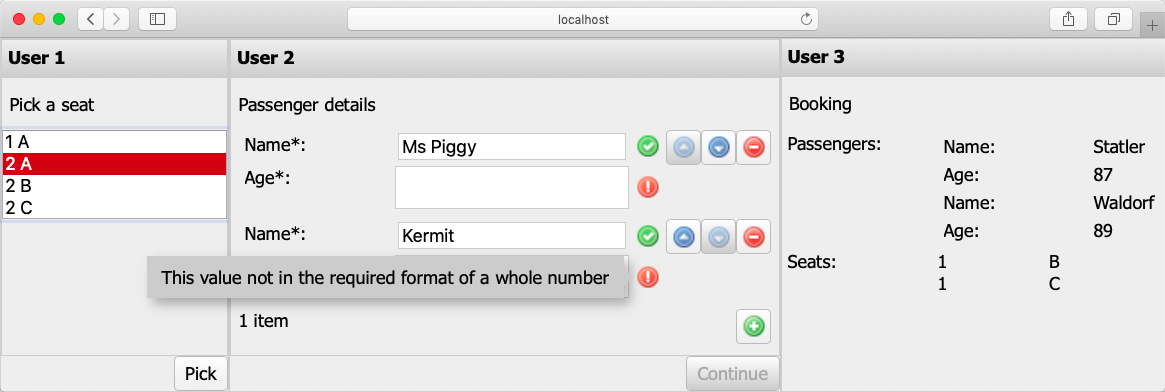
\includegraphics[width=\columnwidth]{figures/flight-booking.png}
  \caption{
    Running web application of the flight booking example using a translation to \ITASKS,
    a \TOP implementation.
    It shows three users booking a flight simultaneously.
    The first user entered name and age and continued to picking seats.
    The second is entering details of two passengers.
    The ages are not filled in, and therefore the \TS{Continue} button is disabled.
    The third user finished a booking.
    Note the first user can't pick seats \smallcaps{1b} and \smallcaps{1c} any more.
    Also, the message bubble shows it is only allowed to enter an integer in the \TS{age} field.
  }
  \label{fig:flight-booking}
\end{figure}

% !TEX root=../pldi2019.tex

\section{System}

\subsection{Base language}
\begin{grammar}
  Expressions
    & e    &::= & \lambda x:\tau.\ e   & – abstraction \\
    &      &\mid& e_1\ e_2             & – application \\
    &      &\mid& x                    & – variable \\
    &      &\mid& c                    & – constant \\
  \addlinespace
    &      &\mid& e_1 \star e_2        & – operate \\
    &      &\mid& \If{e_1}{e_2}{e_3}   & – branch \\
    &      &\mid& \tuple{e_1, e_2}     & – pair \\
    &      &\mid& \unit                & – unit \\
  \addlinespace
  Constants
    & c    &::= & B                    & – boolean \\
    &      &\mid& I                    & – integer \\
    &      &\mid& S                    & – string \\
  \addlinespace
\end{grammar}
\subsection{Editors}
\begin{grammar}
  Expressions
    & e    &::= & p                    & – pretask \\
  Pretasks
    & p    &::= & \Edit e              & – valued editor \\
    &      &\mid& \Enter \beta         & – unvalued editor \\
\end{grammar}
\subsection{Steps}
\begin{grammar}
  Pretasks
    & p    &::= & e_1 \Then e_2        & – step \\
    &      &\mid& e_1 \Next e_2        & – user step
\end{grammar}
\subsection{Composition}
\begin{grammar}
  Pretasks
    & p    &::= & e_1 \And e_2         & – composition \\
  \addlinespace
    &      &\mid& e_1 \Or e_2          & – choice
\end{grammar}
\subsection{State}
\begin{grammar}
  Expressions
    & e    &::= & l                    & – location \\
    &      &\mid& \Ref e               & – reference \\
    &      &\mid& !e                   & – dereference \\
    &      &\mid& e_1 := e_2           & – assign \\
    &      &\mid& e_1; e_2             & – sequence \\
  Pretasks
    & p    &::= & \Update e            & – stored editor \\
\end{grammar}

\begin{mathpar}
  \userule{T-Abs}\qquad
  \userule{T-Var}\\
  \userule{T-If}\\
  \userule{T-App}\qquad
  \userule{T-Ref}\\
  \userule{T-Deref}\qquad
  \userule{T-Loc}\\
  \userule{T-Assign}\qquad
  \userule{T-Pair}\\
  \userule{T-Edit}\\
  \userule{T-Fill}\qquad
  \userule{T-Update} \\
  \userule{T-Fail} \\
  \userule{T-Then} \\
  \userule{T-Next} \\
  \userule{T-And} \\
  \userule{T-Or} \\
  \userule{T-Xor}
\end{mathpar}

% !TEX root=../icfp2019.tex



\section{Semantics}
\label{sec:semantics}

In this section we formalise the semantics of the language constructs described in \cref{sec:language}.
We organise this by following the structure of the language.

Firstly, the task language is embedded in a simply typed lambda calculus.
This requires a specification of the evaluation of terms in the host language, and how it handles the task language.

Secondly, there are two ways to drive evaluation of task expressions, internally by the system itself, and externally by the user.
This is done in two additional semantics, one for the internal normalisation of tasks, and another for the interaction with the end user.

One of our explicit goals is to keep the semantics for evaluation and normalisation separate,
to not mix general purpose programming notions with workflow specific semantics.
This is achieved by letting tasks be values in the host language.

The three main layers of semantics are thus \emph{evaluation}, \emph{normalisation}, and \emph{interaction}.
The semantics, together with \emph{observations}, will be discussed in the following subsections.
\Cref{fig:semantic-functions} shows the relation between the semantics.
It also shows that there are two helper semantics, \emph{handle} and \emph{stride}.

\begin{figure}[h]
  \centering
  \includegraphics[width=0.6\columnwidth,page=5]{figures/drawings-crop.pdf}
  \caption{
    Semantic functions defined in this report and their relation.
  }
  \label{fig:semantic-functions}
\end{figure}

We use the convention that downward arrows are big-step semantics, and rightward arrows are small-step semantics.



\subsection{Evaluating expressions}
\label{sec:evaluation}

The host language evaluates expressions using a big-step semantics.
Evaluating an expression $e$ in state $s$ into a value $v$ in state $s'$ is denoted by $\RelationE$.
To ease reasoning about references, we choose a call-by-value evaluation strategy.

\Cref{fig:value-grammar} shows values with respect to the evaluation semantics.
Tasks are values, and the operands of task constructors are evaluated eagerly.
Exceptions to this are steps and external choice, where some or all of the operands are not evaluated.

\begin{figure}[h]
  \small
  \usemacro{G-Values-Compact}
  \caption{Value grammar} \label{fig:value-grammar}
\end{figure}

The rules to evaluate expressions $e$ do not differ from standard work, except for the task constructs.
The evaluation rules for tasks can be deduced from the value grammar.
They are given in the appendix.

% \begin{figure}[h]
%
%   \begin{gather*}
%     \userule{E-Edit} \Quad
%     \userule{E-Enter} \Quad
%     \userule{E-Update} \Break
%     \userule{E-Then} \Quad
%     \userule{E-Next} \Break
%     \userule{E-And} \Quad
%     \userule{E-Or} \Break
%     \userule{E-Xor} \Quad
%     \userule{E-Appoint} \Quad
%     \userule{E-Fail}
%   \end{gather*}
%
%   \caption{Evaluation semantics for pretasks} \label{}
% \end{figure}


\subsection{Task observations}

% \begin{figure*}[b]
%   \small
%   \usemacro{O-Value-Compact} \hfill \usemacro{O-Failing-Compact} \hfill \usemacro{O-Inputs-Compact}
%   \caption{Values} \label{fig:observation-value}
% \end{figure*}

The normalisation and interaction semantics make use of observations on tasks.
Observations are semantic functions on the syntax tree of tasks.
There are four semantic functions: $\Value$ for the current task value, $\Failing$ to determine if a task fails, $\Inputs$ for the currently accepted input events, and a function for generating user interfaces.
The semantics make use of $\Value$ and $\Failing$, while $\Inputs$ is used for proving safety.
The function for user interfaces is not used by the semantics, but by our implementation.
It is only described in passing here.




\paragraph{Observable values $(\Value)$}

Task values are used by steps to calculate the successor task.
Filled editors are tasks which contain values, as are shared editors.
Unvalued editors do not contain values, neither does the fail task.
These facts propagate through all other task constructors.
The partial function $\Value$ associates a value $v$ to tasks $t$ where possible.
Its definition is given in \cref{fig:observation-value}.

\begin{figure}[h]
  \small
  \usemacro{O-Value}
  \caption{Values} \label{fig:observation-value}
\end{figure}

Internal and external steps do not have an observable value, because calculating the value would require evaluation of the continuation.
Parallel composition only has a value when both branches have values, in which case these values are paired.
Internal choice has a value when one of the branches has a value.
When both branches have a value, it takes the value of the left branch.
External choice does not have a value because it waits for user input.



\paragraph{Failing $(\Failing)$}

In \cref{sub:fail} we introduced $\Fail$ to stand for an impossible task.
Combinations of tasks can also be impossible.
Take for example the parallel composition of two fails ($\Fail \And \Fail$).
This expression is equivalent to $\Fail$, because it can not handle input and can not be further normalised.

This intuition is formalised by the function $\Failing$ in \cref{fig:observation-failing}.
It determines whether a task is impossible.
Such tasks are called \emph{failing}.

\begin{figure}[h]
  \small
  \usemacro{O-Failing}
  \caption{Failing} \label{fig:observation-failing}
\end{figure}

Steps whose left hand sides are failing can never proceed because of the lack of an observable value.
Therefore they are itself failing.
The internal choice of two failing tasks is failing.
External choices let the user pick a side and only then evaluate the corresponding subexpression.
To determine if an external choice is failing, it needs to peek into the future to check if both subexpressions are failing.
Annotations are failing only if the inner task is failing.



\paragraph{User interface}

%\fixme{Add $\UserInterface$ to appendix and refer.}
\TOPHAT is designed such that a user interface can be generated from a task's syntax tree.
A possible graphical user interface is shown in \cref{fig:flight-booking}, where tasks are rendered as \HTML pages.
Editors are rendered as input fields,
external choices are represented by two buttons,
and parallel tasks are rendered side by side.
Steps only show the interface of their left hand side.
In case of an external step they are accompanied by a button.
When the guard condition of a step is not fulfilled, the button is disabled.



\subsection{Normalising tasks}
\label{sec:normalise}

The normalisation semantics is responsible for reducing expressions of type $\Task$ until they are ready to handle input.
It is a big-step semantics, and makes use of evaluation of the host language.
We write $\RelationN$ to describe that
an expression $e$ in state $s$ normalises to task $t$ in state $s'$.

Normalisation rules are given in \cref{fig:normalisation-semantics}.
Both rules ensure that expressions are first evaluated by the host language ($\evaluate$), and then by the stride semantics ($\stride$).
These two actions are repeated until the resulting state and task stabilise.

\begin{figure}[h]
  \small

  \boxed{\RelationN}
  \begin{gather*}
    \userule{N-Done} \Break
    \userule{N-Repeat}
  \end{gather*}
  \caption{Normalisation semantics} \label{fig:normalisation-semantics}

\end{figure}

The split between striding and normalisation is due to mutable references.
Consider the following example, where $s=\set{l\mapsto\False}$.
\begin{TASK}
  (update l >>= \x:Bool. if x then e else fail) <&> (l := True; edit <<>>)
\end{TASK}
\refrule{S-And} reduces this expression in one step to
\begin{TASK}
  (update l >>= \x:Bool. if x then e else fail) <&> (edit <<>>)
\end{TASK}
with $s'=\set{l\mapsto\True}$.
This expression is not normalised, because the left task can take a step.
The issue here lies in the fact that the right task updates $l$.
To overcome this problem, the \refrule{N-Done} and \refrule{N-Repeat} rules ensure that striding is applied until the state $s$ becomes stable and no further normalisation can take place.

The striding semantics is responsible for reducing internal steps and internal choices.
A stride from task $t$ in state $s$ to $t'$ in state $s'$ is denoted by $\RelationS$.
The rules for striding are given in \cref{fig:striding-semantics}.
Tasks like editors, fail and external choice are not further reduced.
For external choice and parallel there are congruence rules.

\begin{figure}[h]
  \small

  \begin{gather*}
    \boxed{\RelationS}
  \end{gather*}

  \paragraph{Step}
  \begin{align*}
    \userule{S-ThenStay} \Quad
    & \userule{S-ThenFail} \Break
    & \userule{S-ThenCont}
  \end{align*}

  \paragraph{Choose}
  \begin{align*}
    \userule{S-OrLeft} \Quad
    & \userule{S-OrRight} \Break
    & \userule{S-OrNone}
  \end{align*}

  \paragraph{Ready}
  \begin{gather*}
    \userule{S-Edit} \Quad \userule{S-Fill} \Quad \userule{S-Update} \Quad
    \userule{S-Fail} \Quad \userule{S-Xor}
  \end{gather*}

  \paragraph{Congruence}
  \begin{gather*}
    \userule{S-Next} \Quad
    \userule{S-And}
    %\userule{S-Appoint}
    % \userule{S-Eval}
  \end{gather*}

  \caption{Striding semantics} \label{fig:striding-semantics}
\end{figure}



\paragraph{Principles of stepping}
\label{sub:stepping-principles}

Stepping away from task $t_1$ can only be performed when
$t_1$ has a value: $\Value(t_1) = v_1$.
Only then can a new task $t_2$ be calculated from the expression $e$.
On top of that, $t_2$ must not be failing: $\neg\Failing(t_2)$.

These principles lead to the stepping rules in \cref{fig:striding-semantics}.
\refrule{S-ThenStay} does nothing,
because the left side does not have a value.
\refrule{S-ThenFail} covers the case that
the left side has a value but the calculated successor task is failing.
This rule uses the semantics of the host language to evaluate the application $e_2\ v_1$.
When all required conditions are fulfilled, \refrule{S-ThenCont} allows stepping to the successor task.



\paragraph{Principles of choosing}
\label{sub:choosing-principles}

Choosing between two tasks $t_1$ and $t_2$ can only be done when
at least one of them has a value: $\Value(t_1) = v_1 \lor \Value(t_2) = v_2$.
When both have a value, the left task is chosen.
When none has a value, none can be chosen.
These principles lead to the rules \refrule{S-OrLeft}, \refrule{S-OrRight}, and \refrule{S-OrNone},
which encode that the choice operator picks the leftmost task that has a value.



\subsection{Handling user inputs}
\label{sec:handling}

The handling semantics is the outermost layer of the stack of semantics.
It is responsible for performing external steps and choices, and for changing the values of editors.
The rules of the interaction semantics are given in \cref{fig:interaction-semantics}.
The semantics is only applicable to normalised $t$.
Sending an input event $i$ to a task $t$ first handles the event and then prepares the resulting task for the next input by normalising it.

\begin{figure}[h]
  \small
  \begin{gather*}
    \boxed{\RelationI} \Break
    \userule{I-Handle}
  \end{gather*}
  \caption{Interaction semantics} \label{fig:interaction-semantics}
\end{figure}

Inputs $i$ are formed according to the grammar in \cref{fig:input-grammar}.
%
There is a function $\Inputs$ which calculates the possible input events a given task expects.
It takes a normalised task and a state and returns a set of inputs that can be handled.
The definition of this function is listed in \cref{fig:observation-input}.

\begin{figure}[h]
  \small
  \usemacro{G-Inputs-Compact}
  \caption{Input grammar} \label{fig:input-grammar}
\end{figure}

\begin{figure}[h]
  \small
  \usemacro{O-Inputs}
  \caption{Inputs} \label{fig:observation-input}
\end{figure}

Handling input is done by the \emph{handling} semantics shown in \cref{fig:handling-semantics}.
It is a small step semantics with labelled transitions.
It takes a task $t$ in a state $s$ and an input $i$, and yields a new task $t'$ in a new state $s'$.

\begin{figure}[h]
  \small

  \begin{gather*}
    \boxed{\RelationH}
  \end{gather*}

  \paragraph{Editing}
  \begin{gather*}
    \userule{H-Change} \Quad
    \userule{H-Empty} \Break
    \userule{H-Fill} \Quad
    \userule{H-Update}
  \end{gather*}

  \paragraph{Continuing}
  \begin{gather*}
    \userule{H-Next} \Break
    \userule{H-PickLeft} \Quad
    \userule{H-PickRight}
  \end{gather*}

  \paragraph{Passing}
  \begin{gather*}
    \userule{H-PassThen} \Quad \userule{H-FirstAnd} \Quad \userule{H-FirstOr} \Break
    \userule{H-PassNext} \Quad \userule{H-SecondAnd} \Quad \userule{H-SecondOr}
  %  \userule{H-Appoint}
  \end{gather*}

  \caption{Handling semantics} \label{fig:handling-semantics}
\end{figure}

%FIXME: Revert rule names in front to normal sentences?
\refrule{H-Change},
\refrule{H-Empty},
\refrule{H-Fill},
\refrule{H-Update}:
Input events $v$ and $\Empty$ are used to change the value of editors and empty them.
Editors only accept values of the correct type.

\refrule{H-Next}:
The $\Continue$(ontinue) action triggers an external step.
As with internal stepping, this is only possible if the left side has a value and the continuation is not failing.

\refrule{H-PickLeft},
\refrule{H-PickRight}:
$\Left$ and $\Right$ are used to pick the left or right option of an external choice.

\refrule{H-PassThen},
\refrule{H-PassNext}:
The step combinators pass all events other than $\Continue$ to the left side.

\refrule{H-FirstAnd},
\refrule{H-SecondAnd},
\refrule{H-FirstOr},
\refrule{H-SecondOr}:
Inputs $\First$(irst) and $\Second$(econd) are used to direct inputs to the correct branch of parallel combinations.



\subsection{Implementation}

The semantics have been implemented in the Idris programming language \cite{journals/jfp/Brady13}.
We use techniques presented by \textcite{journals/entcs/JaskelioffGH11}, \textcite{journals/jfp/Swierstra08}, and \textcite{school/maktoberdorf/PeytonJones01}.
% Such an implementation increases the confidence in the correctness and completeness of the semantics.
The source code can be found on GitHub.\footnote{\url{http://github.com/XXX/XXX}}
% A proof of concept implementation in Haskell is also available, showing that \TOPHAT can be implemented without dependent types.
A command-line interface is part of this implementation.
It prompts users to type input events, which get parsed and processed by the interaction semantics.

Also, we mad an implementation of \TOPHAT combinators into \ITASKS,
so that \TOPHAT specifications can be compiled to runnable applications.
This shows that \TOPHAT is a subset of \ITASKS.

% !TEX root=../icfp2019.tex



\section{Properties}
\label{sec:properties}



% \subsection{Safety}

In order to validate our semantics, we show that our evaluation, normalisation
and handling semantics is type preserving. We additionally prove a progress
theorem for our small-step handling semantics.

Additionally, we show that the normalisation semantics is a big-step semantics.
%XXX: Alejandro: ?
% Niks meer mee doen, was voor PLDI reviewers duidelijk genoeg. --TS
While at first sight, this might seem obvious, the fact that we are dealing with
state complicates matters.

We show that our failing function $\Failing$ indeed only indicates expressions
that can not be normalised and that allow no further interaction.

Finally, we prove that the function to compute all possible inputs $\Inputs$ is sound and complete.



\subsection{Type preservation}
\label{sub:preservation}

We show that the following three preservation Theorems hold.

\begin{theorem}[Type preservation under evaluation]
  % For all well typed expressions $e$ and states $\sigma$,
  For all expressions $e$ and states $\sigma$
  such that $\Gamma,\Sigma \infers e:\tau$ and $\Gamma,\Sigma \infers \sigma$,
  if $e,\sigma \evaluate e',\sigma'$,
  then $\Gamma,\Sigma \infers e':\tau$ and $\Sigma \infers \sigma'$.
  \label{thm:pres-eval}
\end{theorem}

Where $\Sigma \infers \sigma$ means that for all $l\in \sigma$, it holds that
$\Sigma(l)=\Gamma,\Sigma\infers \sigma(l)$.

\Cref{thm:pres-eval} is shown to be correct by induction over $e$. The full
proof can be found in the appendix.


Moving on, we show that normalisation also preserves types, by showing that the following Theorem holds.

\begin{theorem}[Type preservation under normalisation]
  % For all well typed expressions $e$ and states $\sigma$,
  For all expressions $e$ and states $\sigma$
  such that $\Gamma,\Sigma \infers e:\Task\tau$ and $\Sigma \infers \sigma$,
  if $e,\sigma \normalise e',\sigma'$,
  then $\Gamma,\Sigma \infers e':\Task\tau$ and $\Sigma \infers \sigma'$.
  \label{thm:pres-norm}
\end{theorem}

Since this semantics makes use of the value function $\Value$ and the striding semantics $\stride$,
we first need to show that preservation also holds for these two semantics.

\begin{lemma}[Task value preserves types]
  % For all well typed expressions $e$ and states $\sigma$,
  For all expressions $e$ and states $\sigma$
  such that $\Gamma,\Sigma \infers e:\Task\tau$ and $\Sigma \infers \sigma$,
  if $\Value{(e,\sigma)}=v$,
  then $v:\tau$.
  \label{lem:presvalue}
\end{lemma}

\begin{lemma}[Striding preserves types]
  For all expressions $e$ and states $\sigma$
  such that $\Gamma,\Sigma \infers e:\Task\tau$ and $\Sigma \infers \sigma$,
  if $e,\sigma \stride e',\sigma'$,
  then $\Gamma,\Sigma \infers e':\Task\tau$ and $\Sigma \infers \sigma'$.
  \label{thm:pres-stride}
\end{lemma}

\Cref{lem:presvalue} and \cref{thm:pres-stride} are proven in the
appendix by induction over $e$. This subsequently allows us to prove
\Cref{thm:pres-norm}, again by induction over $e$.

This brings us finally to the type preservation property of the handling semantics.

\begin{theorem}[Type preservation under handling]
  % For all well typed expressions $e$, states $\sigma$, and inputs $i$,
  For all expressions $e$, states $\sigma$ and inputs $i$
  such that $\Gamma,\Sigma \infers e:\Task\tau$ and $\Sigma \infers \sigma$,
  if $ e,\sigma \handle{i} e',\sigma'$,
  then $\Gamma,\Sigma\infers e':\Task\tau$ and $\Sigma\infers \sigma'$.
  \label{thm:pres-handle}
\end{theorem}

And again, this is proven by induction over $e$.

From \cref{thm:pres-handle} and \cref{thm:pres-norm} we directly
obtain that the driving semantics also preserves types.

\subsection{Progress}

A well-typed term of a task type is guaranteed to progress after normalisation,
unless it is failing.

We define what we mean with progress in \cref{thm:prog-norm}.
\begin{theorem}[Progress under handling]
  For all well typed expressions $e$ and states $\sigma$,
  % For all expressions $e$ and states $\sigma$
  % such that $\Gamma,\Sigma \infers e:\Task\tau$ and $\Sigma \infers \sigma$,
  if $e,\sigma \normalise e',\sigma'$,
  then either $\Failing(e', \sigma')$
  or there exist $e''$, $\sigma''$, and $i$ such that $e',\sigma'\handle{i} e'',\sigma''$.
  \label{thm:prog-norm}
\end{theorem}

Where a well typed expression $e$ means that $\Gamma,\Sigma\infers e:\tau$ for
some type $\tau$, and a well typed state means that $\Sigma\infers \sigma$.

If an expression $e$ and state $\sigma$ are well-typed, then after normalisation, the pair $e',\sigma'$
either fails, or there exists some input $i$ that can be handled by it under the handling semantics.
In order to prove this Theorem, we require an additional theorem.

% \paragraph{Failing}

We need to show that the failing function $\Failing$ behaves as desired.

\begin{theorem}[Failing means no interaction possible]
  For all well typed expressions $e$ and states $\sigma$,
  % For all expressions $e$ and states $\sigma$
  % such that $\Gamma,\Sigma \infers e:\Task\tau$ and $\Sigma \infers \sigma$,
  and $e,\sigma \normalise e',\sigma'$,
  we have that $\Failing(e',\sigma') = \True$,
  if and only if there is no input $i$
  such that $e',\sigma'\handle{i} e'',\sigma''$ for some $e''$ and $\sigma''$.
  \label{thm:failing}
\end{theorem}

The Theorem above states that an expression $e$ and state $\sigma$ are failing, if,
after normalisation, there exists no input that can be handled by it.
We prove the theorem to be true by induction on $e'$.

% \paragraph{Proof}

We now have the ingredients to prove \cref{thm:prog-norm}.

\begin{proof}
  Given $\Gamma,\Sigma\infers e:\Task\tau$ and $\Sigma\infers \sigma$ and after
  normalisation $e,\sigma \normalise e',\sigma'$, we find ourselves in either one of the
  following situations:

  There exists an $i$ such that $e',\sigma'\handle{i} e'',\sigma''$.

  There does not exist an $i$ such that $e',\sigma'\handle{i} e'',\sigma''$. In this case, we
  know that $\Failing(e',\sigma')$ must be true, by \cref{thm:failing}.
\end{proof}



\subsection{Soundness and Completeness of Inputs}

In order to validate the function that calculates all possible inputs $\Inputs$,
we want to show that the set of possible inputs it produces is both sound and complete with respect to the handle semantics.
By sound we mean that all inputs in the set of possible inputs can actually be handled by the handle semantics,
and by complete we mean that the set of possible inputs contains all inputs that can be handled by the handle semantics.
\Cref{thm:safety-i} expresses exactly this property.

\begin{theorem}[Inputs function is sound and complete]
  For all well typed expressions $e$, states $\sigma$, and inputs $i$,
  % For all expressions $e$, states $\sigma$, and inputs $i$
  % such that $\Gamma,\Sigma \infers e:\tau$ and $\Sigma \infers \sigma$,
  we have that $i \in \Inputs{(e,\sigma)}$ if and only if $e,\sigma \handle{i} e',\sigma'$.
  \label{thm:safety-i}
\end{theorem}

We prove the above theorem by induction over $e$. The proof is listed in the
appendix.

% !TEX root=../pldi2019.tex

\section{Intuition}

This section gives an overview over the essential concepts of \TOP and how they are represented in \TOPHAT.
These concepts are: communication with the environment, communication between subsystems, sequential composition, concurrency, and synchronization.
Many of these concepts are similar in nature to what is commonly found in process algebras.
This raises the question how \TOP and process algebras relate.
While introducing the concepts, we compare them with Hoare's Communicating Sequential Processes (\CSP).
The discussion here is based on the book by \citet{books/Hoare85CSP}.
We chose \CSP as an example to stand for the numerous process algebras in existence, which, as far as this section is concerned, are reasonably similar.

We provide comparisons based on two aspects.
First, we compare the scope of the languages, as intended by the authors.
Second, we show how similar features like concurrency and communication work.


\paragraph{Scope}

The central objective of \TOP is to coordinate the collaboration between people who work together to reach a common goal.
\TOP is a language to specify workflows.

The central objective of \CSP is to model the patters of behaviour of processes.
These patterns of behaviour manifest themselves in sequences of actions that processes can engage in.
\CSP is a language to specify synchronization patterns.

\CSP has a formal semantics that allows various kinds of correctness proofs, including equality of processes, and adherence to a specification.
This allows applications in program correctness, proofs of deadlock freedom, liveness, or verification of protocols.

\TOP focuses less on formal correctness, and more on practical applicability.
It wants to be a language with intuitive semantics that facilitates communication between programmers and domain experts.
\TOP programs are supposed to hide implementation details from domain experts while containing enough information to allow automatic generation of executable applications, including user interfaces.

The big difference between \CSP and \TOP is the intended level of abstraction.
While \CSP is used to explicitly model low-level details about communication, \TOP wants to hide details and provide high-level communication mechanisms to the programmer.

Despite the different origins, \TOP and \CSP feature concepts that serve similar purposes.


\paragraph{Features}

In the rest of this section we focus on features common to \TOP and \CSP, and study their respective realization.
When we point out differences, we do not argue that the different realizations are incompatible.
As a matter of fact the primitives can certainly be expressed in terms of each other.
Instead, we point out how the systems emphasize certain points of view by choosing different building blocks to achieve the same effect.


\subsection{Communication}

Both \TOP and \CSP have two sorts of communication: with the environment, and between subsystems.
In both languages, communication with the environment represents input and output, and blocks evaluation of programs until the environment sends or receives events.
In both languages, communication between subsystems does not block, but evaluates programs as far as possible until further external input is required.

\paragraph{Communication with the environment}
In \TOP, communication with the environment is represented by editors.
A task of the form $\Edit v$, where $v$ is of type $\tau$, can receive any change event with a value of type $\tau$ and additionally the special event $\Empty$ that empties the editor.
The environment can always inspect the current value of an editor.

Editors have no notion of continuation.
Their sole purpose is to interact with the environment, retaining the last value that has been sent to them.

Editors can be used for both input and output.
The interpretation of whether an editor represents input or output is left to the reader.
An empty editor is most commonly interpreted as a prompt to input data, while a filled editor can be seen either as outputting its value, or as an input that comes with a default value.

In \CSP, communication with the environment is represented by prefixing.
The process $(a \to P)$ can engage in action $a$, after which it continues as process $P$.
In general, if $B$ is a set of events and $P(x)$ is an expression that evaluates to a process for each $x \in B$, the process $(x:B \to P(x))$ can engage in any one of the actions in $B$, after which it continues as the process determined by $P(x)$.
Hoare does not specify the language in which $P(x)$ is to be expressed.
He seems to permit any kind of mathematical formula, or any programming language.

Prefixing has no direction of sending and receiving.
Hoare uses the neutral phrase \emph{engaging in an action}.
The interpretation of whether an action stands for input or output is left to the reader.
For example, a vending machine $P = (\textit{coin} \to \textit{choc} \to P)$ is to be interpreted as taking a coin as input and producing chocolate as output.

Sending and receiving of values is modelled by giving additional structure to the names of actions.
For example, an action name could be $\textit{in}.5$, which can be interpreted as inputting the value 5.

In \TOP, event values are typed to match the type of the receiving editor.
In \CSP, action names are essentially strings, subject to implicit restrictions.


\paragraph{Example: vending machine}

This example demonstrates external communication and choice.

The following \CSP program models a vending machine that dispenses a small biscuit for one coin and a large biscuit for two coins. $$V = \textit{coin} \to (\textit{small} \to \text{STOP} \mid \textit{coin} \to \textit{large} \to \text{STOP})$$

A vending machine in \TOP that is close in spirit to the one above looks as follows.
\begin{TASK}
  enter Int >>? \n. if n == 1 then edit "small"
    else if n == 2 then edit "large" else fail
\end{TASK}
This machine does not exhibit exactly the same behaviour as the one in \CSP, nor is it intended to.
Instead, this machine demonstrates how the same choice of buying a small biscuit for one coin or a large biscuit for two coins is expressed in \TOP.

The machine asks the user to enter an amount of money.
This editor stands for a coin slot in a real machine that freely accepts and returns coins.
There is a continue button that is initially disabled.
When the user has input exactly 1 or 2 coins, the continue button becomes enabled.
When the user presses the continue button, the machine dispenses either a large or a small biscuit, depending on the amount of money.


\paragraph{Communication between subsystems}

\TOP has two methods for internal communication, both different from its meth\-od for external communication.
The step combinator represents data flow that follows control flow, and shared data represents data flow across control flow.

The step combinator in $t \Then c$ passes the value of $t$ to the continuation $c$.
Shared data sources are assignable references, whose changes in value are immediately visible to all tasks interested in them.

The semantics of \TOP requires all updates to shared data and all enabled internal steps to be processed before any further communication with the environment can take place.
This introduces the possibility of diverging computations, where a cyclic dependency between shared data causes internal steps to be taken continuously without ever being able to engage in external communication.

\CSP uses prefixing for both internal and external communication.
Parallel processes that all eventually are willing to engage in some action must wait for the others and then progress in one synchronized step.
This step is still visible to the environment, which means the processes can not engage in this action unless the environment is also willing to.
Communication becomes internal by using \emph{concealment}.

Concealment is an operator that hides a given set of actions from the environment, which changes the semantics of prefixing for the concealed actions.
Processes do not have to wait for the environment, they can just step on their own.
In fact, processes must take any concealed steps as soon as possible, before any further communication with the environment can take place.
This means internal steps have priority over external communication.
This introduces the possibility of diverging computations, that is processes which continuously take internal steps without ever being able to engage in external communication.


\paragraph{Sequential composition}

The intuition about sequential composition is to first do one thing, and once it is done, do some other thing.

In \TOP, tasks never terminate.
Nonetheless, the notion of sequential composition exists in two forms: the external and the internal step.
The task $t \Then c$ acts like $t$ as long as the step is guarded.
Once it becomes unguarded, the task continues as $cv$, where $v$ is the value of $t$.
The task $t \Next c$ requires an input event $\Continue$ in addition to the step being unguarded in order to step.

In \CSP, sequential composition is represented by the semicolon combinator together with the special action $\checkmark$, called \emph{success}.
We require that if a process engages in $\checkmark$ at all, it must be its single last action.
When that happens, we say the process terminates successfully.
The process $P;Q$ behaves like $P$ until $P$ terminates successfully, after which it continues as $Q$.
If $P$ never terminates successfully, neither does $P;Q$

\CSP's semicolon is like an internal step $t \Then c$ in \TOP where $t$ uses $\Unit$ to signal when it is done, and $c$ never fails.


\subsection{Multiprogramming}

Both \TOP and \CSP are models of \emph{multiprogramming}, as opposed to multiprocessing.
This means that one processor evaluates multiple programs in an interleaving fashion.
Multiprogramming involves three aspects: concurrency, synchronization, and nondeterminism.

\paragraph{Concurrency}

Concurrency is the source of parallelism: two things are done at the same time.

In \TOP, the parallel combinator $t_1 \And t_2$ stands for two independent tasks carried out at the same time.
For the system it does not matter if the tasks are executed by two people actually in parallel, or by one person who switches between the tasks.
All events sent to the combined task are interleaved into a serial stream of inputs.
The tasks are truly independent of each other, all interleavings are permitted.
Events to $t_1$ and $t_2$ must be prefixed by $\Left$ and $\Right$ respectively.
This unambiguously renames the events, removing any source of nondeterminism.

In \CSP, there are two different combinators for parallel composition: parallel and interleave.
The parallel process $P || Q$ can take $P$-steps and $Q$-steps in arbitrary interleaving for actions unique to $P$ and $Q$.
Actions in the alphabets of both $P$ and $Q$ must be taken in synchronization, so if one process wants to take such a step, it must wait until the other is ready to do so.
Synchronized steps are the only occasion where two processes actually do something at the same time.

The interleaving operator $P ||| Q$ does not synchronize any actions of $P$ and $Q$.
All interleavings are permitted.
Actions that occur in both alphabets are nondeterministically taken by either $P$ or $Q$.


\paragraph{Synchronization}

Synchronization means that an agent has to pause execution until some condition is met.
The need for synchronization arises quite naturally in countless variations in situations involving concurrency.
For multiprogramming, synchronization always means that some of the possible interleavings are forbidden.

For example, the mutual exclusion problem for two parallel processes $a_p \to b_p \to \text{STOP} $ and $a_q \to b_q \to \text{STOP}$ can be stated as:
In no interleaving should there be two adjacent $a$'s.

The mutual exclusion problem for two parallel tasks can be stated as follows.
Let \textit{inc} and \textit{dec} be tasks that increment and decrement some shared counter.
In $(\textit{inc} \Next \textit{dec}) \And (\textit{inc} \Next \textit{dec})$, the shared counter should at no point be greater than 1.
This means that in no interleaving should there be two adjacent \textit{inc}'s.

The basic method for synchronization in \TOP is built into the step combinator.
The task $t \Next c$ can only continue execution when two conditions are met:
Task $t$ must have a value $v$, and $cv$ must not evaluate to $\Fail$.
Programmers can encode arbitrary conditions in $cv$, which are evaluated atomically between interaction steps.
This allows a variety of synchronization problems to be solved in an intuitive and straight-forward manner.

The basic method for synchronization in \CSP is synchronized prefixing.
If some action $a$ is in the alphabets of both $P$ and $Q$, then their parallel composition $P||Q$ can take an $a$-step only if both $P$ and $Q$ are ready to take an $a$-step, in which case they both take their $a$-step simultaneously.
They both have to wait for the condition that the other process is ready to take the step.
All synchronization problems in \CSP must be solved by employing synchronized steps in some form.


\paragraph{Example: Cigarette smokers}

The cigarette smokers problem \cite{books/Downey08LBOS} is a surprisingly tricky synchronization problem.
We study it here because it demonstrates the capabilities of guarded steps.
The problem requires waiting for two conditions, waking up only if both conditions are satisfied.
The problem is stated as follows.
In order to smoke a cigarette, three ingredients are required: tobacco, paper, and a match.
There are three smokers, each having one of the ingredients and requiring the other two.
There is an agent that randomly provides two of the ingredients.

Downey models availability of the ingredients using a semaphore for each ingredient.
The agent randomly signals two of the three semaphores.
The problem asks writing code for the smokers so that the smoker who requires the two signalled semaphores wakes up and proceeds with smoking.

A na\"ive attempt where each smoker first waits for one and then the other semaphore can lead to deadlock.
The following pseudo-code is a non-solution.
Let \emph{paper}, \emph{tobac} and \emph{match} be semaphores, initialized to 0.
\begin{TASK}
  tobacSmoker = wait(match); wait(paper); smoke();
  paperSmoker = wait(tobac); wait(match); smoke();
  matchSmoker = wait(tobac); wait(paper); smoke();
\end{TASK}
To see what can go wrong, imagine the three smokers running in parallel.
Let the agent signal the two semaphores \emph{tobac} and \emph{paper}.
One of \emph{paperSmoker} and \emph{matchSmoker} can take their first step, but if \emph{paperSmoker} takes the step, the system deadlocks.

The solution proposed by Downey involves an additional mutex, three additional semaphores, three additional threads called \emph{pushers}, and three regular Boolean variables.
The job of the pushers is to record availability of their ingredient in their Boolean variable, and check availability of other resources, waking the correct smoker when appropriate.
The details of the solution are not important here.

What is important is that the implementation of what is essentially waiting for two semaphores requires a substantial amount of additional synchronization, together with non-trivial conditional statements.

A similar effort as in Downey's solution must be made in order to solve the problem using synchronized actions in \CSP.
This is because in \CSP, processes can only synchronize on one action at a time.

\TOP allows a simple solution to this problem, using guarded steps.
Steps can be guarded with arbitrary expressions, and the parallel combinator can be used to watch two shared data sources at the same time.
Let \textit{match}, \textit{paper}, and \textit{tobac} be shared Booleans.
The smokers are defined as follows.
\begin{TASK}
  tobacSmoker = (update match <&> update paper) >>? continue
  paperSmoker = (update tobac <&> update match) >>? continue
  matchSmoker = (update tobac <&> update paper) >>? continue
  continue = \<<x,y>>. if x && y then smoke else fail
\end{TASK}
When the agent supplies two of the ingredients by setting the respective shares to $\True$, only the step of the smoker that waits for those becomes enabled.


\paragraph{Nondeterminism}

Nondeterminism means that a system can react to the same input in different ways, the choice of which can not be influenced by the environment.

\CSP has an operator to explicitly introduce nondeterminism.
Furthermore, nondeterminism can arise from the combination of some other combinators, for example choice and concealment.

Hoare states that nondeterminism is only useful for \emph{specifying} processes, never for \emph{implementing} them \cite{books/Hoare85CSP}.
\CSP can be used for both.
A process with nondeterministic behaviour must always be regarded as a specification, while a deterministic process can be seen as specification or implementation.

\TOP is meant solely for implementation and does not have any form of nondeterminism.
Input events for parallel tasks are disambiguated, internal steps have a well-defined evaluation order, and internal choice is left-biased.

% !TEX root=../pldi2019.tex

\section{Conclusion}

\paragraph{Future work}



%% Acknowledgments
\begin{acks}                            %% acks environment is optional
                                        %% contents suppressed with 'anonymous'
  %% Commands \grantsponsor{<sponsorID>}{<name>}{<url>} and
  %% \grantnum[<url>]{<sponsorID>}{<number>} should be used to
  %% acknowledge financial support and will be used by metadata
  %% extraction tools.
  % \footnotesize
  % !TEX root=../icfp2019.tex

The authors are grateful to Johan Jeuring, Sjaak Smetsers, and Andreas Vinter-Hviid for fruitful discussions,
and Rinus Plasmeijer, Peter Achten and Pieter Koopman for proofreading.

This research is supported by the Dutch Technology Foundation STW, which is part
of the Netherlands Organisation for Scientific Research (NWO), and which is
partly funded by the Ministry of Economic Affairs.

\end{acks}


%% Bibliography
\bibliography{bibliography}


%% Appendix
% \appendix
% \section{Appendix}

%Text of appendix \ldots

\end{document}
